\documentclass{article}
\usepackage[utf8]{inputenc}
\usepackage{physics}
\usepackage{amsmath}
\usepackage{showlabels}
\usepackage{amssymb}
\usepackage{natbib}
\usepackage{graphicx}
\usepackage{array}

\renewcommand{\vec}[1]{\ensuremath{\mathbf{#1}}}
\newcommand{\uvec}[1]{\ensuremath{\hat{\mathbf{#1}}}}
\newcommand{\figurewidth}{0.4\textwidth}
\newcommand{\widefigurewidth}{0.8\textwidth}

% One should follow the following naming scheme:
% HW2_SHI_JIALE.zip

\title{Machine Learning\\[1em] Homework 2}
\author{Jiale Shi}
%\date{Dec/10/2018}
\begin{document}
\maketitle

\newpage
\section{Linear Regression}
Consider a data set in which each data point $y_{n}$ is associated with a weighting factor $r_{n}>0$. Therefore, the sum of square error function becomes
\begin{equation}
    E_{D}(\mathbf{w}) = \frac{1}{2} \sum_{n=1}^{N}r_{n}\{y_{n}-\mathbf{w}^{T}\phi(\mathbf{x}_{n})\}^{2}
\end{equation}


Find an expression for the solution $\mathbf{w}^*$ that minimizes this error function. Give two alternative interpretations of the weighted sum-of-squares error function in terms of (a) data dependent noise variance (b) replicated data points.
\\
\textbf{Solution:} \\
\begin{equation}
\begin{aligned}
&  \mathbf{w}^{*}  = {\rm argmin}_{\mathbf{w}}E_{D}(\mathbf{w}) \\
& 0 =  \frac{d E_{D}(\mathbf{w}^{*})}{d \mathbf{w}^{*}}= -\sum_{n=1}^{N}r_{n}\phi(\mathbf{x}_{n})\{y_{n}-\mathbf{w}^{*T}\phi(\mathbf{x}_{n})\} \\
& \sum_{n=1}^{N}r_{n}\phi(\mathbf{x}_{n})\{y_{n}-\mathbf{w}^{*T}\phi(\mathbf{x}_{n})\} = 0
\end{aligned}
\end{equation}
\\
In terms of (a) data dependent noise variance: $E_{D}(\mathbf{w})$ scales the noise of data ($\beta$).
\\
In terms of (b) replicated data points: It shows how many times does each data point is observed.

\newpage
\section{Evidence}
\textbf{A.} In linear regression, the marginal likelihood function is given as 
\begin{equation}
    p(t|\alpha,\beta) = \int p(t|\omega, \beta)p(\omega | \alpha) d\omega
\end{equation}
where
\begin{equation}
    p(\omega | \alpha) = \mathcal{N}(\omega|0,\alpha^{-1} I)
\end{equation}
\begin{equation}
    \log p(t|\omega,\beta) = \sum_{n=1}^{N} \log \mathcal{N}(t_{n}|\omega^{T}\phi(\mathbf{x}_{n}),\beta^{-1})
\end{equation}
\begin{equation}
    E_{D}(\omega) = \frac{1}{2}\sum_{n=1}^{N}\{t -\omega^{T}\phi(\mathbf{x}_{n})\}^{2}
\end{equation}


Using the above equations, derive an expression for the marginal likelihood. \\
\textbf{Solution:} \\
\begin{equation}
\begin{aligned}
& \log p(t|\omega,\beta) = \sum_{n=1}^{N} \log \mathcal{N}(t_{n}|\omega^{T}\phi(\mathbf{x}_{n}),\beta^{-1}) \\
& p(t|\omega,\beta) = \frac{1}{(2\pi)^{N/2}} \beta^{N/2}e^{-\beta E_{D}} \\
& E_{D}(\omega) = \frac{1}{2}\sum_{n=1}^{N}\{t -\omega^{T}\phi(\mathbf{x}_{n})\}^{2}
\end{aligned}
\end{equation}

\begin{equation}
\begin{aligned}
    p(t|\alpha,\beta) & = \int p(t|\omega, \beta)p(\omega | \alpha) d\omega \\
    & = \int \frac{1}{(2\pi)^{N/2}} \beta^{N/2}e^{-\beta E_{D}} \mathcal{N}(\omega|0,\alpha^{-1} I)d\omega  \\
    & = (\frac{\beta}{2\pi})^{N/2}(\frac{\alpha}{2\pi})^{M/2}\int \exp\{-E(\omega)\}d\omega \\
    & = (\frac{\beta}{2\pi})^{N/2}(\frac{\alpha}{2\pi})^{M/2} e^{-E(\mathbf{m}_N)} (2\pi)^{M/2}|\mathbf{A}|^{-1/2}
\end{aligned}
\end{equation}
\begin{equation}
\begin{aligned}
& \mathbf{A} = \alpha \mathbf{I} + \beta \phi^{T}\mathbf{\phi} \\
& E(\mathbf{m}_{N}) = \frac{\beta}{2} ||\mathbf{t}-\mathbf{\phi} \mathbf{m}_{N}||^2 + \frac{\alpha}{2} \mathbf{m}_{N}^{T} \mathbf{m}_{N} \\
& \mathbf{m}_N = \beta \mathbf{A}^{-1}\mathbf{\phi}^{T}\mathbf{t}
\end{aligned}
\end{equation}

\textbf{B.} The conjugate prior for a Gaussian distribution with unknown mean and unknown precision (inverse variance) is a normal-gamma distribution. This property also holds for the case of the conditional Gaussian distribution $p(t|x,\omega,\beta) = \prod^{N}_{n=1} \mathcal{N}(t_{n}|\omega^{T}\phi(x_{n}),\beta^{-1})$ of the linear regression model. If we consider the likelihood function
\begin{equation}
    p(t|x,\omega,\beta) = \prod^{N}_{n=1} \mathcal{N}(t_{n}|\omega^{T}\phi(x_{n}),\beta^{-1})
\end{equation}
then the conjugate prior for $\omega$ and $\beta$ is given by
\begin{equation}
    p(\omega, \beta) = \mathcal{N}(\omega|m_{0}, \beta^{-1}S_{0}) {\rm Gam} (\beta|a_{0},b_{0})
\end{equation}
(a) Show that the corresponding posterior distribution takes the same functional form, so that
\begin{equation}
    p(\omega, \beta | t) = \mathcal{N}(\omega|m_{N}, \beta^{-1}S_{N}) {\rm Gam} (\beta|a_{N},b_{N})
\end{equation} \\
and find expressions for the posterior parameters $\mathcal{m}_{N}$, $S_{N}$, $a_N$ and $b_{N}$.
\\
\textbf{Solution:} \\
\begin{equation}
\begin{aligned}
    p(\omega, \beta | t) & = p(t|x,\omega,\beta)  p(\omega, \beta)  \\
    & = \left\{\prod^{N}_{n=1} \mathcal{N}(t_{n}|\omega^{T}\phi(x_{n}),\beta^{-1}) \right\} \mathcal{N}(\omega|m_{0}, \beta^{-1}S_{0}) {\rm Gam} (\beta|a_{0},b_{0}) \\
    & = \frac{1}{(2\pi)^{N/2}} (\frac{1}{\beta})^{-N/2} \exp \left(-\beta \frac{(\mathbf{y- \Phi w})^{T}(\mathbf{y-\Phi w})}{2} \right)   \\
    & \cdot \frac{b_0^{a_{0}}}{(2\pi)^{D/2}|\mathbf{S}_{0}|^{1/2} \Gamma(a_0)}(\frac{1}{\beta})^{-(a+D/2+1)} \exp \left( -\frac{(\mathbf{w}-m_{0})^{T}(\mathbf{S}_{0})^{-1} (\mathbf{w}-m_{0})+2b}{2\sigma^2}\right) \\
   & = \frac{b_0^{a_{0}}}{(2\pi)^{(N+D)/2}|\mathbf{S}_{0}|^{1/2} \Gamma(a_0)}(\frac{1}{\beta})^{-(a+(D+N)/2+1)}  \\ & \cdot \exp \left( -\beta \frac{(\mathbf{w}-m_{0})^{T}(\mathbf{S}_{0})^{-1} (\mathbf{w}-m_{0})+(\mathbf{y- \Phi w})^{T}(\mathbf{y-\Phi w})+2b_0}{2}\right)
\end{aligned}
\end{equation}


Let us define the following:
\begin{equation}
\begin{aligned}
& \mathbf{S}_{N} = (\mathbf{S}_{0}^{-1} + \mathbf{\Phi^{T}\Phi} )^{-1} \\
& \mathbf{m}_{N} = \mathbf{V}_{N} (\mathbf{S}_{0}^{-1} m_{0} + \mathbf{\Phi^{T}y}) \\
& a_{N} = a_{0} + N/2 \\
& b_{N} = b_{0} + \frac{1}{2} \left(m_{0}\mathbf{S}_{0}^{-1}m_{0} + \mathbf{y^{T}y} - \mathbf{m}_{N} \mathbf{S}_{N} ^{-1} \mathbf{m}_{N}\right) 
\end{aligned}
\end{equation}
with these definitions,

\begin{equation}
\begin{aligned}
    p(\mathbf{w},\sigma^2|D) &   \propto (\frac{1}{\beta})^{-(a_{N}+D/2+1)} \exp \left( -\beta \frac{(\mathbf{w} - \mathbf{m}_{N})^{T}(S_{N})^{-1} (\mathbf{w} - \mathbf{m}_{N})^{T}+2b_{N}}{2}\right) \\
    & = \mathcal{N} (\mathbf{w}| \mathbf{m}_{N},\beta^{-1} \mathbf{S}_{N}) {\rm Gam} (\beta| a_{N},b_{N}) 
\end{aligned}
\end{equation}
\\
(b) Show that the marginal probability of the data (model evidence) is given by
\begin{equation} 
\begin{aligned}
    p(t) = \frac{1}{2\pi^{N/2}}\frac{b_{0}^{a_{0}}}{b_{N}^{a_{N}}} \frac{|S_{N}|^{1/2}}{|S_{0}|^{1/2}} \frac{\Gamma(a_{N})}{\Gamma(a_{0})}
\end{aligned}
\end{equation}
\\
\textbf{Solution:}
\begin{equation} 
\begin{aligned}
    p(t) & =   \int \int p(t|x,\omega,\beta) p(\omega, \beta) dw d\beta 
\end{aligned}
\end{equation}

\newpage
\section{Mixture of conjugate priors}
\textbf{A.} Show that a mixture of conjugate priors is indeed a conjugate prior.\\
\textbf{Solution: }
From Murphy's book, 5.4.4 mixture of conjugate priors.
We can represent a mixture of conjugate priors by introducing a latent indicator variable $z$, where $z = k$ means that $\theta$ comes from mixture component $k$. The prior has the form
\begin{equation}
p(\theta) = \sum_{k=1}^mp(z=k)p(\theta|z=k)
\end{equation}

Then the posterior can be written as 
\begin{equation}
p(\theta | D) = \frac{p(D | \theta)  p(\theta)}{p(D)}
\end{equation}

Combine the above two equations

\begin{equation}
p(\theta | D) =  \sum_{k=1}^m \frac{1}{p(D)} p(z=k)p(\theta|z=k)p(D | \theta)
\end{equation}

And, if we know $\theta$, no matter what the $z$ is, $p(D | \theta)$ won't change. Therefore,
$p(D |\theta) = p(D |\theta, z=k)$.

\begin{equation}
\begin{aligned}
 p(\theta | D) & =  \sum_{k=1}^m \frac{p(z=k)}{p(D)} p(\theta|z=k)p(D |\theta, z=k) \\
 &  = \sum_{k=1}^m \frac{p(D | z = k) p(z=k)}{p(D)} \frac{p(\theta|z=k)p(D |\theta, z=k)}{p(D | z = k)}
 \\
& =  \sum_{k=1}^m \frac{p(D | z = k) p(z=k)}{p(D)} p(\theta | D, z = k) \\
& = \sum_{k=1}^m p(z = k | D) p(\theta | D, z = k)
\end{aligned}
\end{equation}
$p(z = k | D)$ is the posterior weight. $\sum_{k=1}^{m} p(z = k | D)= 1 $ 
\\
\textbf{B.} Suppose we use the mixture prior $p(\theta) = 0.5 {\rm Beta}(\theta|a_{1},b_{1})+0.5 {\rm Beta}(\theta|a_{2},b_{2})$, where $a_{1}=b_{1} = 20$, $a_{2}=b_{2} = 10$ and we observe $N_{1}$ head and $N_{0}$ tails. Derive an expression and write a computer code for evaluating the posterior. Consider $N_{1} = 20$ heads and $N_{0}=10$ tails. Show with a plot a comparison between the prior and the posterior.
\begin{figure}[h!]
\centering
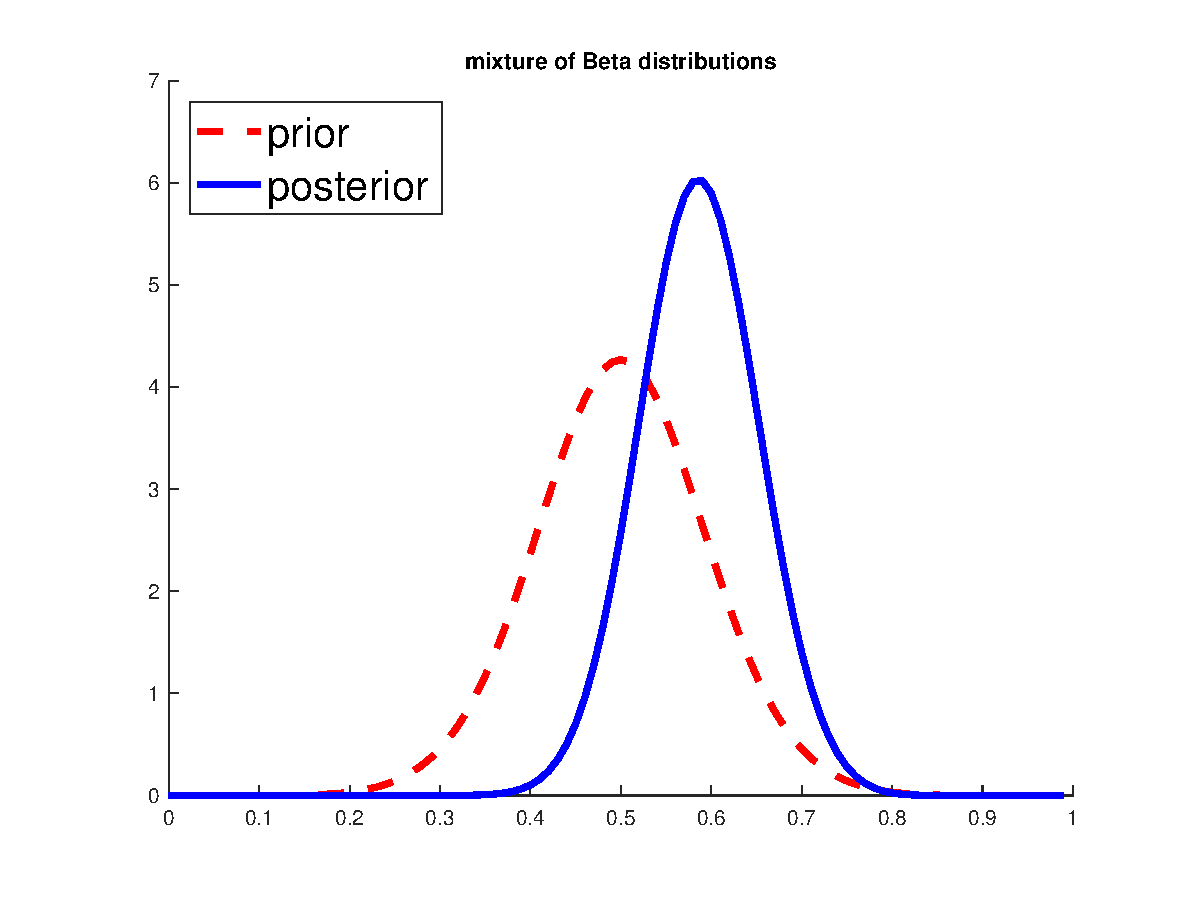
\includegraphics[width=\widefigurewidth]{fig/P3b.eps}
\caption{Comparison between the prior and the posterior}
%\label{fig:universe}
\end{figure}



\newpage
\section{Optimal threshold on classification probability}
Consider a case where we have learned a conditional probability distribution $p(y|x)$. Suppose there are only two classes, and let $p_{0} = p(y=0|x)$ and $p_{1} = p(y=1|x)$. Consider the loss matrix shown in Table 1.

\textbf{A. } Show that the decision $\hat{y}$ that minimizes the expected loss is equivalent to setting a probability threshold $\theta$ and predicting $\hat{y} =0$ if $p_{1} < \theta$ and $\hat{y} = 1$ if $p_{1} \geq \theta$. Derive $\theta$ as a function of $\lambda_{01}$ and $\lambda_{10}$.\\
\textbf{Solution:}\\
\begin{equation}
\begin{aligned}
& p_0 = p(y=0|\mathbf{x}) \\
& p_1 = p(y=1|\mathbf{x}) \\
& p_0 + p_1 = 1 \\
& p_0 = 1-p_1
\end{aligned}
\end{equation}

predicting $\hat{y} = 0$ if $p_1 <\theta$ and $\hat{y} = 1$ if $p_1 >\theta$ 

$L_{FN} = \lambda_{01}$ and $L_{FP} = \lambda_{10}$ \\
One should pick the class $\hat{y}=1$ if 
\begin{equation}
\begin{aligned}
& \frac{p_1}{p_0} > \frac{ \lambda_{10}}{\lambda_{01}} \\
& \frac{p_1}{1-p_1} > \frac{ \lambda_{10}}{\lambda_{01}} \\
& p_1 > \frac{\frac{\lambda_{10}}{\lambda_{01}}}{1+ \frac{\lambda_{10}}{\lambda_{01}}}
\end{aligned}
\end{equation}
Therefore,
\begin{equation}
    \theta =  \frac{\frac{\lambda_{10}}{\lambda_{01}}}{1+ \frac{\lambda_{10}}{\lambda_{01}}}
\end{equation}
\textbf{B. } Derive the loss function where the threshold is 0.1. \\
\textbf{Solution:} \\
From part \textbf{A}
\begin{equation}
    0.1 = \theta =  \frac{\frac{\lambda_{10}}{\lambda_{01}}}{1+ \frac{\lambda_{10}}{\lambda_{01}}}
\end{equation}\\

\begin{equation}
 \frac{\lambda_{10}}{\lambda_{01}} = \frac{1}{9}
\end{equation}

if $p_1 <0.1$,  $\hat{y} = 0$ 
\begin{equation}
    L = p_1 \lambda_{01}
\end{equation}

and if $p_1 >0.1$, $\hat{y} = 1$ 
\begin{equation}
    L = p_0 \lambda_{10}
\end{equation}

%5
\newpage
\section{Bayes Factor}
\textbf{A. } Suppose we toss a coin $N$ times and observe $N_{1}$ heads. Let $N_{1} \sim {\rm Bin}(N,\theta)$ and $\theta \sim {\rm Beta}(1,1)$. Show that the marginal likelihood is $p(N_{1}|N) = \frac{1}{N+1}$.
\\
\textbf{Solution:}\\
\begin{equation}
\begin{aligned}
p(\theta|\mathcal{D}) & = \frac{p(\theta) p(\mathcal{D}|\theta)}{p(\mathcal{D})} \\ 
 & = \frac{1}{p(\mathcal{D})}\left[\frac{1}{B(a,b)} \theta^{a-1}(1-\theta)^{b-1}\right] \left[\left( \begin{array}{c}  N \\  N_1
    \end{array} \right) \theta^{N_1} (1-\theta)^{N_0}\right] \\
\end{aligned}
\end{equation}

\begin{equation}
\begin{aligned}
\frac{1}{B(a+N_1,b+N_0)} & = \frac{1}{p(\mathcal{D})}\frac{1}{B(a,b)} \left( \begin{array}{c}  N \\  N_1 \end{array} \right)
\end{aligned}
\end{equation}

\begin{equation}
\begin{aligned}
p(N_{1}|N) = p(\mathcal{D}) & = \left( \begin{array}{c}  N \\  N_1 \end{array} \right)    \frac{B(a+N_1,b+N_0)}{B(a,b)} \\
& =  \left( \begin{array}{c}  N \\  N_1 \end{array} \right)    \frac{B(1+N_1,1+N_0)}{B(1,1)}
& = \frac{N!}{N_1 ! N_0 !} \frac{\frac{N_1 ! N_0 !}{(N+1)!}}{\frac{0! 0!}{1!}} \\
& = \frac{1}{N+1}
\end{aligned}
\end{equation}

\textbf{B. } Suppose we toss a coin $N = 10$ times and observe $N_{1} = 9$ heads. Let the null hypothesis be that the coin is fair, and the alternative be that the coin can have any bias, so $p(\theta) = \mathcal{U}(0,1)$. Derive the Bayes factor $BF_{0,1}$ in favor of the biased coin hypothesis. What if $N = 100$ and $N_{1} = 90$? \\
\textbf{Solution:}\\
If the coin is fair
\begin{equation}
    P_0(N_1 | N) = \left( \begin{array}{c}  N \\  N_1 \end{array} \right) (0.5)^{N_1}(0.5)^{N_0} =  \left( \begin{array}{c}  N \\  N_1 \end{array} \right) (0.5)^{N}
\end{equation} 
\\
If the coin can have any bias, from part A
\begin{equation}
\begin{aligned}
p_1(N_{1}|N) = p(\mathcal{D}) = \frac{1}{N+1}
\end{aligned}
\end{equation}

\begin{equation}
   BF_{0,1} = \frac{P_0(N_1 | N)}{\frac{1}{N+1}}  = \left( \begin{array}{c}  N \\  N_1 \end{array} \right) (0.5)^N (N+1)
\end{equation}\\
Therefore, if we toss a coin $N = 10$ times and observe $N_{1} = 9$ heads,

\begin{equation}
   BF_{0,1} =  \left( \begin{array}{c}  10 \\  9 \end{array} \right) (0.5)^{10} (10+1) = \frac{55}{512} = 0.1074
\end{equation}
\\
Therefore, if we toss a coin $N = 100$ times and observe $N_{1} = 90$ heads,

\begin{equation}
   BF_{0,1} =  \left( \begin{array}{c}  100 \\  90 \end{array} \right) (0.5)^{100} (100+1) = 1.379\times10^{-15}
\end{equation}

\newpage
\section{Behavior of training set error with increasing sample size, Multi-out regression and Ridge regression}
\textbf{A. } The error on the test will always decrease as we get more training data, since the model will be better estimated. However, for sufficiently complex models, the error on the training set can increase as we get more training data, until we reach some plateau. Explain why.
\\
\textbf{Solution:}\\
When the training data is not enough, these complex models are easy to be overfitting, which would leads to very low training error and very high test error. \\
For example, the true function is very complex. But when there are only two points, we get a linear model and the training error is 0 while the test error is very large. However, when we get more training data, the model begins to learn from the training data and becomes more and more close to the true function. As a result, the training error and test error would converge to one same plateau. Therefore, as we get more training data, the training error can increase and the test error would decrease.
\\
\textbf{B. } When we have multiple independent outputs in linear regression, the model becomes
\begin{equation}
    p(\mathbf{y}|\mathbf{x}, \mathbf{W}) = \prod_{j=1}^{M} \mathcal{N}(y_{j}|w_{j}^{T}\mathbf{x}_{i},\sigma_{j}^{2})
\end{equation}
Since the likelihood factorizes across dimensions, so does the MLE. Thus,
\begin{equation}
    \hat{W} = [\hat{w}_{1},...,\hat{w}_{M}]
\end{equation}
where $\hat{w}_{j} = (X^{T}X)^{-1}X^{T} Y_{:,j}$.

In this exercise, we apply this result to a model with 2 dimensional response vector $y_{i} \in \mathbb{R}^2$. Suppose we have some binary input data $x_{i} \in \{0,1\}$. The training data is as follows. Let us embed each $x_{i}$ into 2d using the following basis function

\begin{equation}
    \phi(0) = (1,0)^{T}, \phi(1) = (0,1)^{T},
\end{equation}

The model becomes 
\begin{equation}
    \hat{\mathbf{y}} = W^{T}\phi(x)
\end{equation}
where $W$ is a $2\times2$ matrix. Compute the MLE for $W$ from the above data. \\
\textbf{Solution:} \\
\begin{equation}
\begin{aligned}
& \hat{\mathbf{y}} = W^{T}\phi(x) \\
& y_{j} = \phi(x)^{T}\mathbf{w}_{j} \\
& y_1 = \phi(x)^{T} \mathbf{w}_1 
& y_2 = \phi(x)^{T} \mathbf{w}_2
\end{aligned}
\end{equation}

\begin{equation}
\begin{aligned}
&\mathbf{w}_1  = \left[\begin{array}{c}  a \\  b \end{array} \right] 
&\mathbf{w}_2 = \left[\begin{array}{c}  c \\  d \end{array} \right] 
\end{aligned}
\end{equation}
\\
Using the least squares to minimize the sum squares error function $L_{s}$.
\begin{equation}
\begin{aligned}
L_s = & (-1-a)^2+(-1-c)^2 \\
     & + (-1-a)^2+(-2-c)^2 \\
     & + (-2-a)^2+(-1-c)^2 \\
     & + (1-b)^2+(1-d)^2 \\
     & +(1-b)^2 + (2-d)^2 \\
     & +(2-b)^2 + (1-d)^2
\end{aligned}
\end{equation}
when $a=-\frac{4}{3}$, $b=\frac{4}{3}$, $c=-\frac{4}{3}$, $d=\frac{4}{3}$, $L_s$ gets the minimum value.
There,

\begin{equation}
\begin{aligned}
&\mathbf{w}_1  = \left[\begin{array}{c}  -\frac{4}{3} \\  \frac{4}{3} \end{array} \right]  
&\mathbf{w}_2 = \left[\begin{array}{c}  -\frac{4}{3} \\  \frac{4}{3} \end{array} \right]  \\
& \mathbf{W} = [\mathbf{w}_1, \mathbf{w}_2] =  \left[\begin{array}{cc}  -\frac{4}{3} & -\frac{4}{3} \\  \frac{4}{3} & \frac{4}{3} \end{array} \right]
\end{aligned}
\end{equation}
\\
\textbf{C. } Assume that $\hat{x} = 0$, so that the input data is centered. Show that the optimizer (in case of ridge regression) of 
\begin{equation}
    J(\mathbf{w},w_{0}) = (\mathbf{y} - X\mathbf{w} - w_{0} \mathbf{1})^{T}(\mathbf{y} - X\mathbf{w} - w_{0} \mathbf{1})+ \lambda \mathbf{w}^{T}\mathbf{w}
\end{equation}
is
\begin{equation}
    w_{0} = \bar{y}
\end{equation}

\begin{equation}
    \mathbf{w} = (\mathbf{X}^{T}\mathbf{X}+\lambda \mathbf{I})^{-1}\mathbf{X}^{T} \mathbf{y}
\end{equation}
\\
\textbf{Solution:}\\
\begin{equation}
\begin{aligned}
    & 0 = \frac{d J}{ d w_{0}} = 2N w_{0} + 2(\mathbf{X}\mathbf{w}-\mathbf{y})^{T}\mathbf{1} \\
    & w_{0} = \bar{y} - \mathbf{W}\hat{x}
\end{aligned}
\end{equation}
Since the problem assume that $\hat{x} = 0$, therefore, $\mathbf{W}\hat{x} = 0$
\begin{equation}
\begin{aligned}
& w_{0} = \bar{y}
\end{aligned}
\end{equation}

\begin{equation}
    0 = \frac{d J}{ d \mathbf{w}} = 2 \mathbf{X}^{T} \mathbf{X} \mathbf{w} - 2\lambda \mathbf{w} - \mathbf{X}^{T} \mathbf{X} + 2 w_{0} \mathbf{X}^{T} \mathbf{1}
\end{equation}
Since the problem assume that $\hat{x} = 0$, therefore, $\mathbf{X}^{T} \mathbf{I}= 0$
\begin{equation}
\begin{aligned}
&0 = 2 \mathbf{X}^{T} \mathbf{X} \mathbf{w} + 2\lambda \mathbf{I} \mathbf{w} - 2\mathbf{X}^{T} \mathbf{y} \\
& \mathbf{w} = (\mathbf{X}^{T}\mathbf{X}+\lambda \mathbf{I})^{-1}\mathbf{X}^{T} \mathbf{y}
\end{aligned}
\end{equation}
\\
\textbf{D. } For the data set provided, we want to fit a linear regression model with polynomial order $M$. In this regard, perform the following tasks:
\\
(a) Compute the unknown coefficients based on MLE with $M = 2,4,10,14$. Compute and plot the mean square error for the training and the test set corresponding to various polynomial orders.\\
\textbf{Solution:}\\
\begin{figure}[h!]
\centering
\includegraphics[width=\widefigurewidth]{fig/P6da.eps}
\caption{Mean Square Error for the training and test set corresponding to various polynomial orders based on MLE}
%\label{fig:universe}
\end{figure}\\
From the results, we find that when polynomial order is 10, the mean square error for the test set is smallest.\\
(b) Compute the known coefficients based on ridge regression and plot the fitted function. Report the mean square error corresponding to the training and the test set.\\
\textbf{Solution:}\\
We set  polynomial order is 10 and compute the unknown coefficients based on ridge regression.
The fitted functions corresponding to different lambdas are
\begin{figure}[h!]
\centering
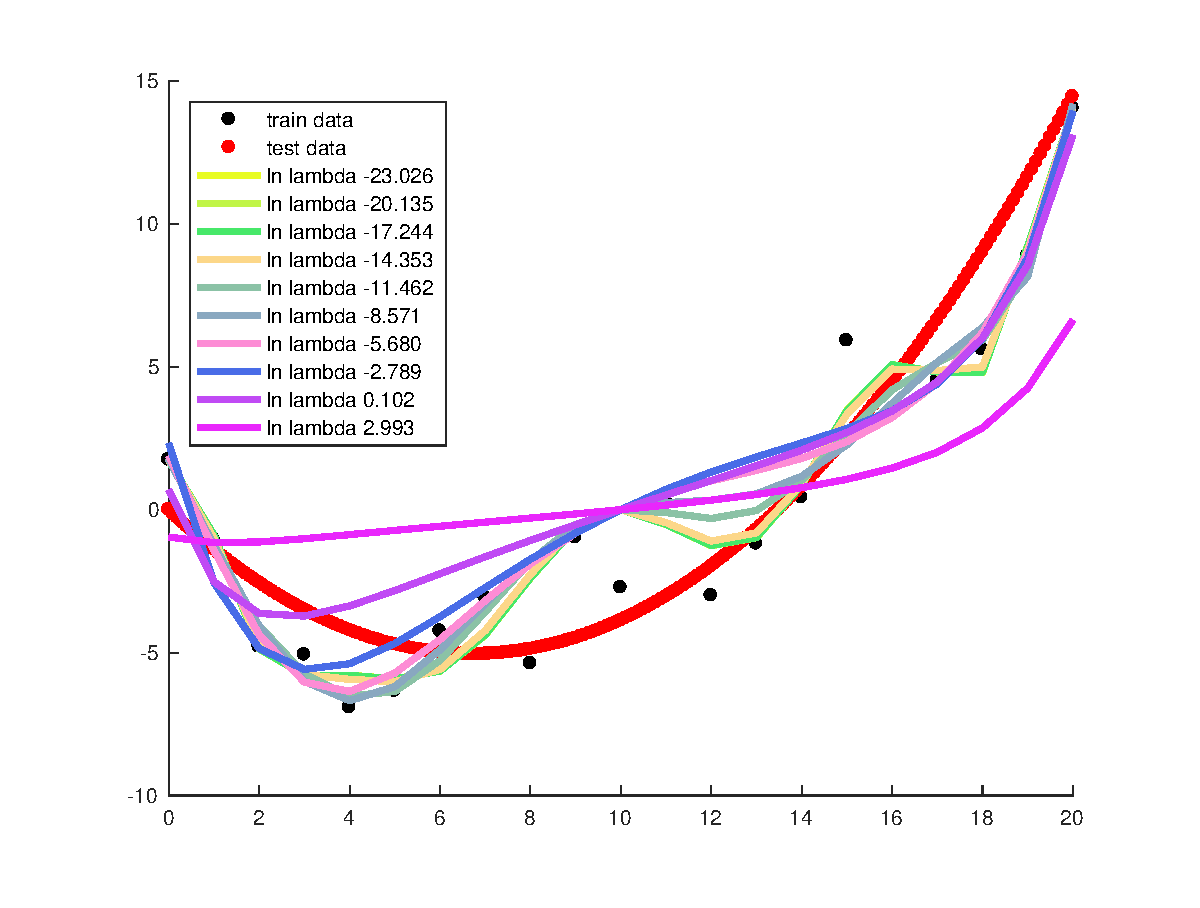
\includegraphics[width=\widefigurewidth]{fig/P6db1.eps}
\caption{The fitted functions corresponding to different lambdas}
%\label{fig:universe}
\end{figure}
Instead of reporting the mean square error, it is clearer to show the mean square error in the figure.
\begin{figure}[h!]
\centering
\includegraphics[width=\widefigurewidth]{fig/P6db.eps}
\caption{Mean Square Error for the training and test set corresponding to various lambdas with polynomial order is 10 based on redge regression}
%\label{fig:universe}
\end{figure} \\
When $\log(\lambda) = -14.3528$, the test error is smallest.

\newpage
\section{Bayesian linear regression}
We consider a Bayesian linear regression model to fit a set of points $x^{i}$,$y^i$,$i=1,...,N$ data points with up to order $M=5$  polynomials. For your implementation consider the data provided. The data is generated using the following data generation algorithm:
\\
$x=10\* \rm rand(N,1)$; generate input points \\
noise = 3\*randn(N,1); generate Gaussian noise \\
$y=(x-4)^2+\rm noise$; actual truth function \\
The particulars of the regression model are given below:
\begin{equation}
    p(\mathbf{y}|\mathbf{\Phi}, \mathbf{w},\sigma^2) = \mathcal{N}(\mathbf{y}|\mathbf{\Phi}\mathbf{w},\sigma^2\textbf{I}_{N})
\end{equation}
where $\mathbf{\Phi}$ is the design matrix. The prior to be considered is as follows:
\begin{equation}
    p(\mathbf{w}|\sigma^2,\mathbf{\Phi}) = \mathcal{N}(0,\gamma \sigma^2 \mathbf{I})
\end{equation}
where $p(\sigma^2) = {\rm InvGamma}(a,b)$. The particular parameter that you should use in your implementation are $a = 0.1$, $b = 0.00001$ and $\gamma = 0.001/N$
\\
\textbf{A.} Derive an expression for the posterior of $p(\mathbf{w},\sigma^2|D)$, the marginal posterior $p(\mathbf{w}|D)$, predictive distribution $p(y|x,D)$ and the model evidence $p(D)$. \\
\textbf{Solution:} \\
\begin{equation}
\begin{aligned}
   &  p(\mathbf{w},\sigma^2|D)  = p(\mathbf{y}|\mathbf{\Phi}, \mathbf{w},\sigma^2) (p(\mathbf{w}|\sigma^2,\mathbf{\Phi}) \cdot p(\sigma^2) ) \\
    & = \mathcal{N}(\mathbf{y}|\mathbf{\Phi}\mathbf{w},\sigma^2\textbf{I}_{N}) \mathcal{N}(0,\gamma \sigma^2 \mathbf{I}) {\rm InvGamma}(a,b)  \\
    &  = \frac{1}{(2\pi)^{N/2}} (\sigma^2)^{-N/2} \exp \left(-\frac{(\mathbf{y- \Phi w})^{T}(\mathbf{y-\Phi w})}{2\sigma^2} \right)   \\
    & \cdot \frac{b^a}{(2\pi)^{D/2}|\gamma I|^{1/2} \Gamma(a)}(\sigma^2)^{-(a+D/2+1)} \exp \left( -\frac{\mathbf{w}^{T}(\gamma I)^{-1} \mathbf{w}+2b}{2\sigma^2}\right) \\
   & = \frac{b^a}{(2\pi)^{(N+D)/2}|\gamma I|^{1/2} \Gamma(a)}(\sigma^2)^{-(a+(D+N)/2+1)} \exp \left( -\frac{\mathbf{w}^{T}(\gamma I)^{-1} \mathbf{w}+(\mathbf{y- \Phi w})^{T}(\mathbf{y-\Phi w})+2b}{2\sigma^2}\right)
\end{aligned}
\end{equation}
Let us define the following:
\begin{equation}
\begin{aligned}
& \mathbf{V}_{N} = ((\gamma I)^{-1} + \mathbf{\Phi^{T}\Phi} )^{-1} \\
& \mathbf{w}_{N} = \mathbf{V}_{N} ((\gamma I)^{-1} w_{0} + \mathbf{\Phi^{T}y})  =\mathbf{V}_{N} ( \mathbf{\Phi^{T}y}) \\
& a_{N} = a + N/2 \\
& b_{N} = b + \frac{1}{2} (w_{0}(\gamma I)^{-1}w_{0} + \mathbf{y^{T}y} - \mathbf{w}_{N}^{T} \mathbf{V}_{N} ^{-1} \mathbf{w}_{N}) \\ 
& = b + \frac{1}{2} ( \mathbf{y^{T}y} - \mathbf{w}_{N}^{T} \mathbf{V}_{N} ^{-1} \mathbf{w}_{N})
\end{aligned}
\end{equation}
with these definitions,
\begin{equation}
\begin{aligned}
    p(\mathbf{w},\sigma^2|D) &   \propto (\sigma^2)^{-(a+(D+N)/2+1)} \exp \left( -\frac{(\mathbf{w} - \mathbf{w}_{N})^{T}(V_{N})^{-1} (\mathbf{w} - \mathbf{w}_{N})^{T}+2b}{2\sigma^2}\right)
\end{aligned}
\end{equation}

\begin{equation}
\begin{aligned}
    p(\mathbf{w}|D) & \propto \int_{0}^{\infty} \propto (\sigma^2)^{-(a+(D+N)/2+1)} \exp \left( -\frac{(\mathbf{w} - \mathbf{w}_{N})^{T}(V_{N})^{-1} (\mathbf{w} - \mathbf{w}_{N})^{T}+2b}{2\sigma^2}\right) d(\sigma)^2 \\
    & \propto \left[1+\frac{(\mathbf{w} - \mathbf{w}_{N})^{T}(V_{N})^{-1} (\mathbf{w}-\mathbf{w}_{N})}{2b_{N}} \right]^{ - \frac{2a_{N}+D}{2}} \\
    & = \mathcal{T}_{D} (\mathbf{w}, \frac{b_{N}}{a_{N}}\mathbf{V_{N}},2a_{N})
\end{aligned}
\end{equation}
\newpage
\begin{equation}
\begin{aligned}
    p(y|x,D) = \mathcal{T}_{m} (\mathbf{y} | \mathbf{\Phi}\mathbf{w}, \frac{b_{N}}{a_{N}}(\mathbf{I}_{m}+\mathbf{\Phi} \mathbf{V}_{N} \mathbf{\Phi}^{T}),2a_{N})
\end{aligned}
\end{equation}
\newpage
\begin{equation}
\begin{aligned}
    p(D) = \frac{1}{(2\pi)^{N}} \frac{|\mathbf{V}_{N}|^{1/2}}{|\gamma \mathbf{I}|^{1/2}} \frac{b^a}{b_{N}^{a_{N}}} \frac{\Gamma(a_{N})}{\Gamma(a)}
\end{aligned}
\end{equation}
\newpage
\textbf{B.} For polynomial orders $M = 1,2,3,4,5$ plot the predictive mean and the predictive error bars. Your plots should also indicate the exact function as well as the training data points. \\
\textbf{Solution:} \\
\begin{equation}
\begin{aligned}
& \mathbf{V}_{N} = ((\gamma I)^{-1} + \mathbf{\Phi^{T}\Phi} )^{-1} \\
& \mathbf{w}_{N} = \mathbf{V}_{N} ((\gamma I)^{-1} w_{0} + \mathbf{\Phi^{T}y})  =\mathbf{V}_{N} ( \mathbf{\Phi^{T}y}) \\
& a_{N} = a + N/2 \\
& b_{N} = b + \frac{1}{2} (w_{0}(\gamma I)^{-1}w_{0} + \mathbf{y^{T}y} - \mathbf{w}_{N}^{T} \mathbf{V}_{N} ^{-1} \mathbf{w}_{N}) \\ 
& = b + \frac{1}{2} ( \mathbf{y^{T}y} - \mathbf{w}_{N}^{T} \mathbf{V}_{N} ^{-1} \mathbf{w}_{N})
\end{aligned}
\end{equation}
\\
the predictive mean is $\mathbf{\Phi} \mathbf{w}_N$ \\
the predictive variance matrix is $\frac{b_{N}}{a_{N}}(\mathbf{I}_m + \mathbf{X}\mathbf{V}_{N}\mathbf{X}^{T})$ \\
the predictive error bar is the square root of diagonal value of  the predictive variance matrix. \\
\begin{figure}[h!]
\centering
\includegraphics[width=\widefigurewidth]{fig/P7b1.png}
\caption{Predictive mean and the predictive error bars for polynomials $M = 1,2,3,4,5$}
%\label{fig:universe}
\end{figure}

\newpage
\textbf{C. } Draw samples of $\mathbf{w}$ and for each of them show the predictive mean. What additional information this graph provides that is not given in your plots in B above?\\
\textbf{Solution:} \\
\begin{equation}
\begin{aligned}
    p(\mathbf{w}|D) & = \mathcal{T}_{D} (\mathbf{w}, \frac{b_{N}}{a_{N}}\mathbf{V_{N}},2a_{N}) \\ & \propto \left[1+\frac{(\mathbf{w} - \mathbf{w}_{N})^{T}(V_{N})^{-1} (\mathbf{w}-\mathbf{w}_{N})}{2b_{N}} \right]^{ - \frac{2a_{N}+D}{2}}
\end{aligned}
\end{equation}
Therefore, we need to draw samples from multi-variable Student's T distribution.

\begin{figure}[h!]
\centering
\includegraphics[width=\widefigurewidth]{fig/P7c.png}
\caption{Draw samples of $\mathbf{w}$ from Student T distribution $M = 1,...,5$}
%\label{fig:universe}
\end{figure}

\newpage
\textbf{D. } Show a plot comparing the model evidence for polynomials $M = 1, ..., 5$ and select the best model represents the training data. \\
\textbf{Solution:} \\
\begin{figure}[h!]
\centering
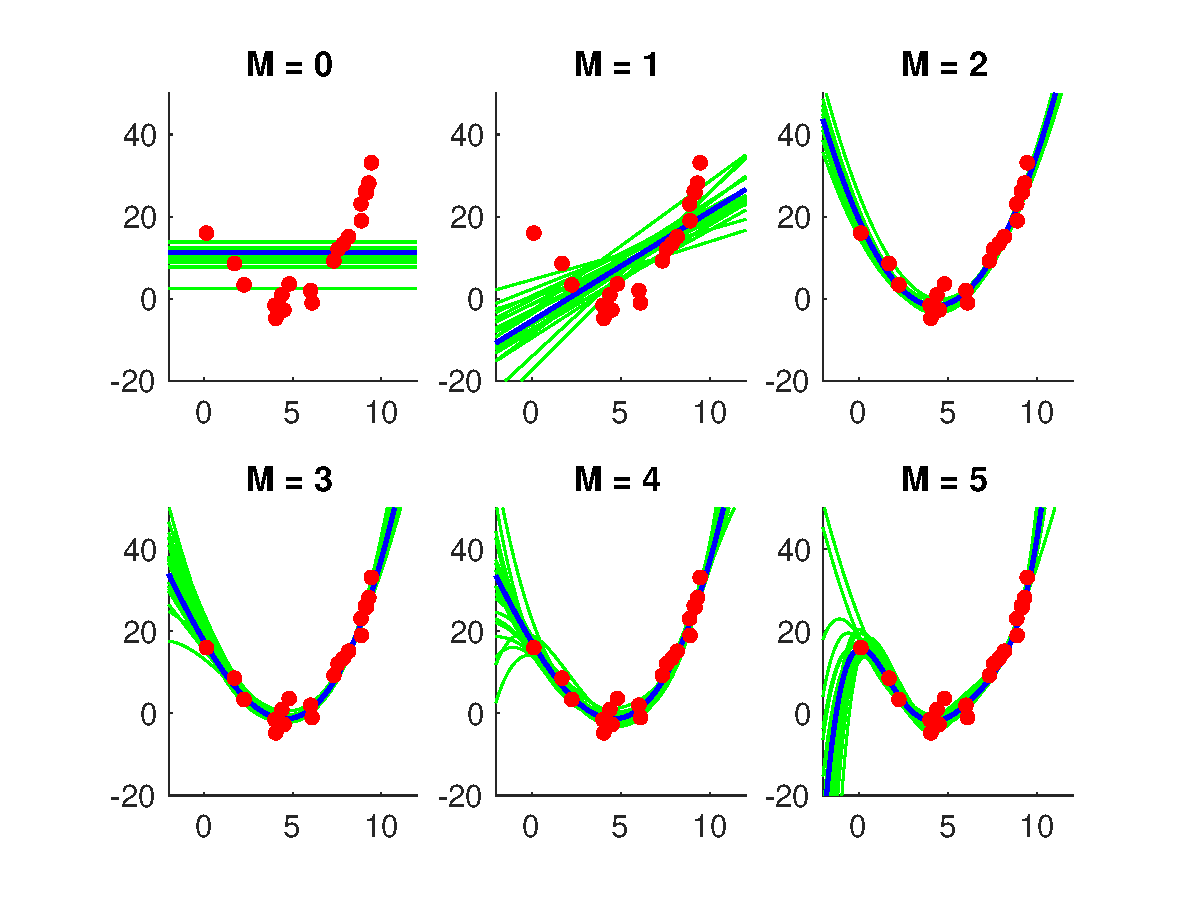
\includegraphics[width=\widefigurewidth]{fig/P7d1.eps}
\caption{Bayesian model comparison for polynomials $M = 1,...,5$}
%\label{fig:universe}
\end{figure}\\

\begin{figure}[h!]
\centering
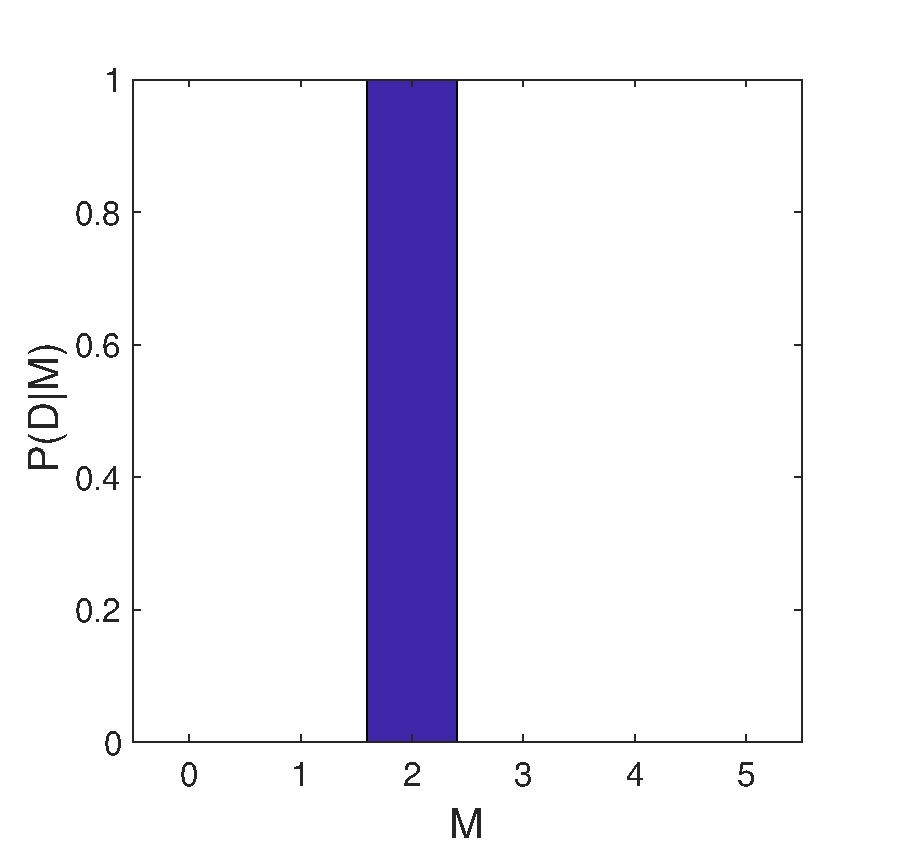
\includegraphics[width=\figurewidth]{fig/P7d2.eps}
\caption{Model evidence for polynomials $M = 1,...,5$}
%\label{fig:universe}
\end{figure}

We are looking for the order of the polynomial that maximizes the model evidence. Therefore, we select $M =2$ that best represents the training data. 
\newpage
\textbf{E. } In Bayesian regression we should not regularize the bias term. This can be easily accomplished by using centered input ($\mathbf{\Phi}$) and output data ($\mathbf{y}$). The bias term can be computed and added to your solution through a post-processing operation. Using such a procedure, repeat the plot in B above for the optional model selected in B.\\
\textbf{Solution:}  \\
From the notes, first, we use centered input ($\mathbf{y}$) \\
$y \rightarrow y-\bar{y}$ \\
The $X$ don't have the constant term.
Then we do the same procedure as B.
\\
Then we can $w$.
In order to get $w_{0}$, 
\begin{equation}
    w_{0} = \bar{y} - \bar{X}^{T}w
\end{equation}

From B, we find that $M=4$ is the optimal model.
Therefore, we repeat $M=4$

\begin{figure}[h!]
\centering
\includegraphics[width=\widefigurewidth]{fig/P7e.png}
\caption{Predictive mean and the predictive error bars for polynomials $M = 4$}
%\label{fig:universe}
\end{figure}


%\bibliographystyle{plain}
%\bibliography{references}
\end{document}
